\documentclass[spanish,12pt,a4paper,titlepage]{report}
%\usepackage[latin1]{inputenc}
\usepackage[utf8]{inputenc}
\usepackage{graphicx}
\usepackage{subfig}
\usepackage{float}
\usepackage{wrapfig}
\usepackage{multirow}
\usepackage{caption}
\usepackage[spanish]{babel}
\usepackage[dvips]{hyperref}
\usepackage{amssymb}
\usepackage{listings}
\usepackage{epsfig}
\usepackage{amsmath}
\usepackage{array}
\usepackage[table]{xcolor}
\usepackage{multirow}
\usepackage{hhline}
\usepackage{cancel}
%\usepackage[Sonny]{fncychap}
%\usepackage[Glenn]{fncychap}
\usepackage[Conny]{fncychap}
%\usepackage[Rejne]{fncychap}
%\usepackage[Bjarne]{fncychap}
\usepackage{subfiles}
\usepackage{framed}
\usepackage{appendix}
\setlength{\topmargin}{-1.5cm}
\setlength{\textheight}{25cm}
\setlength{\oddsidemargin}{0.3cm} 
\setlength{\textwidth}{15cm}
\setlength{\columnsep}{0cm}
\begin{document}
\subfile{portada}
\subfile{introduccion}
\part{Descripción del sistema}
\subfile{general}
\subfile{hardware}
\part{Modelado del sistema}
\subfile{modelo_fisico}
\subfile{simulador}
\part{Motores}
\subfile{sniffer}
\subfile{test_motores}
\part{Calibración y caracterizaci\'on de los sensores}
\subfile{acc_mongoose}
\subfile{gyro_mongoose}
\subfile{magnetometro}
\subfile{barometro}
\subfile{gps}
\part{Estimaci\'on del estado}
\subfile{kalman}
\part{Desarrollo del controlador}
\subfile{linealizacion}
\subfile{control}
\subfile{sim_control}
\subfile{test_control}

\cleardoublepage
\addappheadtotoc
\renewcommand{\appendixpagename}{Anexos}
\appendixpage
\renewcommand{\appendixname}{Anexo}
\renewcommand{\appendixtocname}{Anexo}


\appendix %Tuve que ponerlos con include porque con el subfile quedaban todos numerados con A
\documentclass[main]{subfiles}

\begin{document}

\chapter{Especificaciones t\'ecnicas de la Mongoose 9DoF IMU}
\label{chap:anexo_mongoose}
\section{Aceler\'ometro}

\begin{table}[H]
\begin{center}
\rowcolors{1}{gray!20}{}
\begin{tabular}{|p{3cm}|p{6.5cm}|}
\hline
Rango & $\pm$16g \\
\hline
Resoluci\'on & 10-13 bits (siempre 4mg/LSB) \\
\hline
Datos nuevos &  0.1 a 800 Hz\\
\hline
Ru\'ido XY & 0.75@100Hz - 3@3200Hz LSB-rms\\
\hline
Ru\'ido Z & 1.1@100Hz - 4.5@3200Hz LSB-rms\\
\hline
Cross Axis & $\pm$ 1\% \\
\hline
\end{tabular}
\label{tab:acc-anexo}
\end{center}
\end{table}

\textbf{NOTAS}:
\begin{itemize}
\item Output data rate puede llegar a 3200Hz, pero usando SPI. Con I$^2$C a 400kHz solamente se puede llegar a 800Hz.
\item Ancho de banda = $Datos\_nuevos/2$
\end{itemize}

\section{Gir\'oscopo}

\begin{table}[H]
\begin{center}
\rowcolors{1}{gray!20}{}
\begin{tabular}{|p{3cm}|p{6.5cm}|}
\hline
Rango & $\pm$2000$^\circ/s$ \\
\hline
Resoluci\'on & 14.475 LSB/($^\circ/s$) \\
\hline
Datos nuevos &  3.9Hz a 8kHz\\
\hline
Ancho de banda & 256Hz \\
\hline
Cross Axis & $\pm$ 2\% \\
\hline
Ru\'ido & 0.38 $^\circ/s$-rms \\
\hline
\end{tabular}
\label{tab:gyro}
\end{center}
\end{table}

\textbf{NOTAS}:
\begin{itemize}
\item Datos nuevos: La muestras pasan por un LPF digital de 256 a 5Hz, esto limita el ancho de banda.
\end{itemize}

\section{Magnet\'ometro}

\begin{table}[H]
\begin{center}
\rowcolors{1}{gray!20}{}
\begin{tabular}{|p{3cm}|p{6.5cm}|}
\hline
Rango & $\pm$8 Ga\\
\hline
Resoluci\'on &  5mGa@GN=2\\
\hline
Datos nuevos &  0.75 - 75Hz\\
\hline
Ancho de banda &  37Hz\\
\hline
Cross Axis & $\pm$0.2\% FS/Ga \\
\hline
Ru\'ido & - \\
\hline
\end{tabular}
\label{tab:magn}
\end{center}
\end{table}

\newpage
\textbf{NOTAS}:
\begin{itemize}
\item El rango queda determinado por la ganancia, que se configura con 3 bits:
\begin{table}[H]
\begin{center}
\rowcolors{1}{gray!20}{}
\begin{tabular}{|c|c|c|c|c|c|c|c|c|}
\hline
\textbf{GN} & 0 & 1 & 2 & 3 & 4 & 5 & 6 & 7 \\
\textbf{Rango} (Ga)& $\pm$0.88 & $\pm$1.3 & $\pm$1.9 & $\pm$2.5 & $\pm$4.0 & $\pm$4.7 & $\pm$5.6 & $\pm$8.1 \\
\hline
\end{tabular}
\label{tab:magn-gain}
\end{center}
\end{table}
\item Se puede configurar para que el dato que muestre sea el promedio de hasta 8 muestras.
\end{itemize}

\section{Sensor de presi\'on}

\begin{table}[H]
\begin{center}
\rowcolors{1}{gray!20}{}
\begin{tabular}{|p{3cm}|p{6.5cm}|}
\hline
Rango & 300 a 1100 hPa (9000 a -500m)\\
\hline
Resoluci\'on &  1Pa\\
\hline
Precisi\'on. Abs. & typ/max $\pm$1.0/$\pm$3.0 hPa \\
\hline
Precisi\'on Rel. & $\pm$0.5 hPa \\
\hline
Datos nuevos &  typ/max: 3/4.5ms - 17/25ms\\
\hline
Ancho de banda &  333/40Hz\\
\hline
Ru\'ido (hPa) &  0.06 - 0.03\\
\hline
Ru\'ido (m) & 0.5 - 0.25 \\
\hline
\end{tabular}
\label{tab:barometro}
\end{center}
\end{table}

\textbf{NOTAS}:
\begin{itemize}
\item El rango, en altura, se refiere a la altura sobre el nivel del mar.
\item El modo de operaci\'on (cantidad de muestras promediadas) afecta:
  \begin{itemize}
  \item El tiempo de conversi\'on.
  \item El ancho de banda.
  \item La resoluci\'on.
  \item El ru\'ido.
  \end{itemize}
\item Es necesario hacer una medida de temperatura de vez en cuando (1Hz) para mejorar la lectura del sensor de presi\'on.
\end{itemize}

\section{Sensor de temperatura}

\begin{table}[H]
\begin{center}
\rowcolors{1}{gray!20}{}
\begin{tabular}{|p{3cm}|p{6.5cm}|}
\hline
Rango & 0 a 65 $^\circ$C\\
\hline
Resoluci\'on &  0.1 $^\circ$C\\
\hline
Precisi\'on Abs. & typ/max $\pm$1.0/$\pm$2.0 $^\circ$C\\
\hline
Datos nuevos &  typ/max: 3/4.5ms\\
\hline
Ru\'ido & - \\
\hline
\end{tabular}
\label{tab:temp}
\end{center}
\end{table}

\textbf{NOTAS}:
\begin{itemize}
\item El sensor de temperatura est\'a incorporado al sensor de presi\'on.
\end{itemize}

\end{document}
\documentclass[main]{subfiles}
\begin{document}

%\appendix


\chapter{Cálculo de los tensores}
\label{chap:anexo_tensores}

\section{Magnitudes a considerar}
Según el modelo considerado explicado en \ref{chap:modelo} dividiremos el sistema en una esfera central, cuatro cilindros y cuatro varillas (también cilíndricas). Las magnitudes que debemos conocer para calcular los momentos de inercia del sistema son:

\begin{itemize}
\item Radio de la esfera central $R=8\times10^{-2}m$
\item Largo de las varillas $L=26\times10^{-2}m$
\item Radio de los motores $r=1.65\times10^{-2}m$
\item Altura de los motores $h=3.5\times10^{-2}m$
\end{itemize}

Además nos interesa conocer las distancias de cada uno de los elementos del sistema al centro de masa del cuadricóptero.

\begin{itemize}
\item Distancia entre el centro de masa de la varilla y el centro de masa del cuadricóptero $d_v=14\times10^{-2}m$
\item Distancia del eje de los motores al centro de masa del cuadricóptero $d_m=0.29m$
\end{itemize}

Por último las masas de los elementos en cuestión son:

\begin{itemize}
\item Masa de la esfera central $M_E=1.037kg$
\item Masa de las varillas $M_v=0.013kg$
\item Masa de los motores $M_m=0.113kg$
\end{itemize}



\section{Tensor de inercia del sistema}

\label{tensores}

El tensor de inercia del sistema puede calcularse como la suma de los tensores de inercia de los rígidos que lo componen. Se considera como fue expresado anteriormente el centro del cuadricóptero como una esfera maciza. El tensor de inercia de dicha esfera puede calcularse a partir de la definición misma de tensor de inercia, sin embargo por ser una forma geométrica de vasto uso en el campo de la mecánica su tensor de inercia se encuentra ya tabulado. Sucede lo mismo con las restantes formas geométricas que componen al sistema. Los tensores utilizados pueden obtenerse en \cite{bib:inercia} En el caso de la esfera se tiene que el tensor de inercia respecto de  su centro de masa es: 

$$
\Pi_{G_E}^{\{\vec{i_q}, \vec{j_q}, \vec{k_q}\}}= M_E\left(\begin{array}{ccc}
\frac{2R^2}{5}  &0&  0\\
0  &\frac{2R^2}{5} & 0\\
0  &0 & \frac{2R^2}{5} \\
\end{array}\right) \\
$$

En este caso el centro de masa del sistema corresponde al centro de masa de la esfera a partir de ciertas suposiciones que se realizan sobre la simetría del sistema. Por dicho motivo podemos afirmar que $\Pi_{G_E}^{\{\vec{i_q}, \vec{j_q}, \vec{k_q}\}} = \Pi_{O\prime _E}^{\{\vec{i_q}, \vec{j_q}, \vec{k_q}\}} $, siendo $O\prime$ el centro de la esfera.

Por otra parte el tensor de inercia de una varilla, cuya longitud coincide con el versor $\vec{i_q}$, respecto a su centro de masa tiene la forma:

$$
\Pi_{G_{Vx}}^{\{\vec{i_q}, \vec{j_q}, \vec{k_q}\}}= M_V\left(\begin{array}{ccc}
0  &0&  0\\
0  &\frac{L^2}{12} & 0\\
0  &0 & \frac{L^2}{12}  \\
\end{array}\right) \\ 
$$

Sin embargo resulta mucho ms interesante obtener el tensor de inercia expresado respecto del centro de masa del sistema. Para realizar dicho cambio se utiliza el Teorema de Steiner. Dicho teorema afirma que: $\Pi_Q = \Pi_G +J_Q^{M,G}$, donde los términos de $J_Q^{M,G}$ pueden calcularse como: $(J_Q^{M,G})_{\alpha \beta} = M(G-Q)^2\delta_{\alpha \beta}-M(G-Q)_{\alpha}M(G-Q)_{\beta}$. El término $\delta_{\alpha \beta}$ es conocido como Delta de Kronecker. Su valor es uno si $\alpha =\beta$ y cero si $\alpha \neq \beta$. En el caso en consideración dicha matriz resulta en:

$$
J_O\prime^{M_{Vx},G}= M_V \left(\begin{array}{ccc}
0  &0&  0\\
0  & (\frac{L}{2}+d_v)^2 & 0\\
0  &0 & (\frac{L}{2}+d_v)^2  \\
\end{array}\right) \\
$$

Por lo tanto el momento de inercia total de dicha varilla es:
$$
\Pi_{O\prime_{Vx}}^{\{\vec{i_q}, \vec{j_q}, \vec{k_q}\}}=M_V \left(\begin{array}{ccc}
0  &0&  0\\
0  &\frac{L^2}{3}+(\frac{Ld_v}{2})^2+d_v^2 & 0\\
0  &0 & \frac{L^2}{3}+(\frac{Ld_v}{2})^2+d_v^2  \\
\end{array}\right)$$


Análogamente, el tensor de inercia de una varilla cuya longitud se encuentra respecto de la dirección $\vec{j_q}$ respecto del centro de masa del sistema es:

$$
\Pi_{O\prime_{Vy}}^{\{\vec{i_q}, \vec{j_q}, \vec{k_q}\}}=M_V \left(\begin{array}{ccc}
\frac{L^2}{3}+(\frac{Ld_v}{2})^2+d_v^2  &0 & 0\\
0  &0 & 0\\
0  &0 & \frac{L^2}{3}+(\frac{Ld_v}{2})^2+d_v^2  \\
\end{array}\right)$$


Sucede algo similar en lo que respecta a los motores. Tendremos un tensor de inercia para los motores que se encuentran sobre la dirección $\vec{i_q}$ y otro para los motores que se encuentran sobre la dirección $\vec{j_q}$. El momento de inercia de un cilindro en su centro de masa es:

\begin{equation}
\label{eq:izzm}
\Pi_{G_{M}}^{\{\vec{i_q}, \vec{j_q}, \vec{k_q}\}}=M_M\left(\begin{array}{ccc}
\frac{3r^2+h^2}{12}  &0&  0\\
0  &\frac{3r^2+h^2}{12} & 0\\
0  &0 & \frac{r^2}{2}  
\end{array}\right)
\end{equation}
La entrada $(3,3)$ de la matriz de la ecuación \ref{eq:izzm} la pasaremos a llamar $I_{zzm}$\\

Por lo tanto el momento de inercia respecto del centro de masa del sistema para un cilindro que se encuentra en la dirección $\vec{i_q}$ es:
$$
\Pi_{O\prime_{Mx}}^{\{\vec{i_q}, \vec{j_q}, \vec{k_q}\}}=M_M\left(\begin{array}{ccc}
\frac{3r^2+h^2}{12}  &0&  0\\
0  &\frac{3r^2+h^2}{12} +d_m^2& 0\\
0  &0 & \frac{r^2}{2}+d_m^2  
\end{array}\right)
$$


En el caso de un cilindro que se encuentra en la dirección $\vec{j_q}$ se tiene que::
$$
\Pi_{O\prime_{My}}^{\{\vec{i_q}, \vec{j_q}, \vec{k_q}\}}=M_M\left(\begin{array}{ccc}
\frac{3r^2+h^2}{12} +d_m^2 &0&  0\\
0  &\frac{3r^2+h^2}{12} & 0\\
0  &0 & \frac{r^2}{2}+d_m^2  
\end{array}\right)
$$


Finalmente, el tensor de inercia del sistema, se calcula como la suma de los tensores de inercia de las partes que lo componen:
$$\Pi_{O\prime}^{\{\vec{i_q}, \vec{j_q}, \vec{k_q}\}} =\Pi_{O\prime_E}^{\{\vec{i_q}, \vec{j_q}, \vec{k_q}\}} + 2 \Pi_{O\prime_{Vx}}^{\{\vec{i_q}, \vec{j_q}, \vec{k_q}\}} + 2 \Pi_{O\prime_{Vy}}^{\{\vec{i_q}, \vec{j_q}, \vec{k_q}\}} + 2 \Pi_{O\prime_{Mx}}^{\{\vec{i_q}, \vec{j_q}, \vec{k_q}\}}+ 2 \Pi_{O\prime_{My}}^{\{\vec{i_q}, \vec{j_q}, \vec{k_q}\}}$$.

Dado que todos los tensores de inercia considerados hasta el momento son diagonales, podemos escribir el tensor de inercia del sistema como:

$$\Pi_{O\prime}^{\{\vec{i_q}, \vec{j_q}, \vec{k_q}\}}=\left(\begin{array}{ccc}
I_{xx}  &0&  0\\
0  &I_{yy}& 0\\
0  &0 & I_{zz}  
\end{array}\right)$$

\section{Resultados} 

En base al análisis realizado hasta el momento se tiene que: 

$$I_{zmm}=1.54\times10^{-5}kgm^2
$$

$$
I_{xx}=I_{yy}=2.32\times10^{-2}kgm^2
$$

$$
I_{zz}=4.37\times10^{-2}kgm^2
$$
\end{document}
 
%\documentclass[main]{subfiles}
%\begin{document}

%\appendix

%\cleardoublepage
%\addappheadtotoc
%\appendixpage
%\renewcommand{\appendixname}{Anexo}
%\renewcommand{\appendixtocname}{Anexo}
%\renewcommand{\appendixpagename}{Anexos}
\chapter{C\'alculos necesarios para la linealizaci\'on del sistema}
\label{chap:anexo_linealizacion}

Tal como se explica en el cap\'itulo \ref{chap:linealizacion} se lineliza el MVE obtenido en \ref{chap:modelo}, esto es, aproximar el sistema no lineal por un sistema lineal de la forma:

\begin{equation}
\dot{\tilde{X}}(t)=A(t)\tilde{X}(t)+B(t)\tilde{u}(t)
\end{equation}
Donde $A(t)$ y $B(t)$ son tales que $a_{ij}= \frac{\partial f_i}{\partial x_j}\vert_{u=u^*}^{x=x^*}$ y  $b_{ij}= \frac{\partial f_i}{\partial u_j}\vert_{u=u^*}^{x=x^*}$

\section{Linealizaci\'on para cualquier trayectoria}

Para una trayectoria gen\'erica al linealizar el sistema se obtienen las matrices:

\begin{equation}
\label{eq:Agenerica}
A(t)=\left(\begin{array}{cccc}
0 & A_{12} & A_{13} & 0 \\
0 & A_{22} & 0      & A_{24}\\
0 & A_{32} & A_{33} & A_{34}\\
0 & A_{42}     & 0      & A_{44} \\    
\end{array}\right)
\end{equation}\\


\begin{equation}
\label{eq:Bgenerica}
B(t)=\left(\begin{array}{c}
0\\
0\\
B_{31}\\
B_{41} 
\end{array}\right)
\end{equation}\\
Las entradas de la matriz de \ref{eq:Agenerica} representan matrices de $3\times3$ mientras que las entradas de la matriz \ref{eq:Bgenerica} representan matrices de $3\times4$. Es importante conocer las entradas de las matrices anteriores, al menos en lo que respecta a las dependencias de cada una de ellas con las variables de estado. 

\begin{equation}
A_{12}=\left(\begin{array}{ccc}
f_{A_{12_1}}(\psi,\varphi,\theta,v_{qy},v_{qz}) & f_{A_{12_2}}(\psi,\varphi,\theta,v_{qx},v_{qy},v_{qz}) &  f_{A_{12_3}}(\psi,\varphi,\theta,v_{qx},v_{qy},v_{qz}) \\
f_{A_{12_4}}(\psi,\varphi,\theta,v_{qy},v_{qz}) & f_{A_{12_5}}(\psi,\varphi,\theta,v_{qx},v_{qy},v_{qz}) & f_{A_{12_6}}(\psi,\varphi,\theta,v_{qx},v_{qy},v_{qz}) \\
f_{A_{12_7}}(\psi,\varphi,v_{qy},v_{qz})&                                                        f_{A_{12_8}}(\psi,\varphi,v_{qx},v_{qy},v_{qz})&                                                                                                                                                 0\\
\end{array}\right)
\end{equation}\\

\begin{equation}
A_{13}=\left(\begin{array}{ccc}
f_{A_{13_1}}(\psi,\varphi,\theta) & f_{A_{13_2}}(\psi,\varphi,\theta) &  f_{A_{13_3}}(\psi,\varphi,\theta) \\
f_{A_{13_4}}(\psi,\varphi,\theta) & f_{A_{13_5}}(\psi,\varphi,\theta) & f_{A_{13_6}}(\psi,\varphi,\theta) \\
f_{A_{13_7}}(\varphi)& f_{A_{13_8}}(\psi,\varphi)&                                                                                                                                                 f_{A_{13_8}}(\psi,\varphi)\\
\end{array}\right)
\end{equation}\\

\begin{equation}
A_{22}=\left(\begin{array}{ccc}
f_{A_{22_1}}(\psi,\varphi,\omega_{qy},\omega_{qz}) & f_{A_{22_2}}(\psi,\varphi,\omega_{qy},\omega_{qz}) &  0 \\
f_{A_{22_4}}(\psi,\omega_{qy},\omega_{qz}) & 0 & 0 \\
f_{A_{22_7}}(\psi,\varphi,\omega_{qy},\omega_{qz})&                                                        f_{A_{22_8}}(\psi,\varphi,\omega_{qy},\omega_{qz})&                                                                                                                                                 0\\
\end{array}\right)
\end{equation}\\

\begin{equation}
A_{24}=\left(\begin{array}{ccc}
1 & f_{A_{24_2}}(\psi,\varphi) & f_{A_{24_3}}(\psi,\varphi) \\
0 & f_{A_{24_5}}(\psi) & f_{A_{24_6}}(\psi) \\
0&f_{A_{24_8}}(\psi,\varphi)&f_{A_{24_9}}(\psi,\varphi)\\
\end{array}\right)
\end{equation}\\

\begin{equation}
A_{32}=\left(\begin{array}{ccc}
0 & g\cos \varphi & 0 \\
-g\cos \varphi \cos \psi & g\sin\varphi\sin\psi & 0 \\
 g\cos \varphi \sin \psi & g\sin\varphi\cos\psi & 0 \\
\end{array}\right)
\end{equation}\\

\begin{equation}
A_{33}=\left(\begin{array}{ccc}
0 & \omega_{qz} & -\omega_{qy} \\
-\omega_{qz} & 0 &\omega_{qx} \\
\omega_{qy} & -\omega_{qx}& 0 \\
\end{array}\right)
\end{equation}\\

\begin{equation}
A_{34}=\left(\begin{array}{ccc}
0 & -v_{qz} & v_{qy} \\
v_{qz} & 0 &-v_{qx} \\
-v_{qy} & v_{qx}& 0 \\
\end{array}\right)
\end{equation}\\

\begin{equation}
A_{42}=Mgd\left(\begin{array}{ccc}
-\frac{\cos\varphi\cos\psi}{I{xx}} & \frac{\sin\varphi\sin\psi}{I{xx}} & 0 \\
0 & -\frac{\cos\phi}{I{yy}} &0 \\
0 & 0& 0 \\
\end{array}\right)
\end{equation}\\

\begin{equation}
A_{44}=\left(\begin{array}{ccc}
0 &\frac{I_{zzm}}{I_{xx}}(\omega_1-\omega_2+\omega_3-\omega_4) + \frac{I_{yy}-I_{zz}}{I_{xx}}\omega_{qz}& \frac{I_{yy}-I_{zz}}{I_{xx}}\omega_{qy} \\
\frac{I_{zzm}}{I_{yy}}(\omega_1-\omega_2+\omega_3-\omega_4) + \frac{-I_{xx}+I_{zz}}{I_{yy}}\omega_{qz} & \frac{-I_{xx}+I_{zz}}{I_{yy}}\omega_{qx}\\
0&0&0\\
\end{array}\right)
\end{equation}\\

\begin{equation}
B_{31}=\left(\begin{array}{cccc}
0 & 0 & 0 &0\\
0&0&0\\
f_{B_{31_9}}(\omega_1) & f_{B_{31_10}}(\omega_2) & f_{B_{31_11}}(\omega_3) &f_{B_{31_12}}(\omega_4)\\
\end{array}\right)
\end{equation}\\

\begin{equation}
B_{41}=\left(\begin{array}{cccc}
0 & f_{B_{41_2}}(\omega_2) & 0 & f_{B_{41_4}}(\omega_4)\\
f_{B_{41_5}}(\omega_1)&0&f_{B_{41_6}}(\omega_3)&0\\
f_{B_{41_9}}(\omega_1) & f_{B_{41_10}}(\omega_2) & f_{B_{41_11}}(\omega_3) &f_{B_{41_11}}(\omega_4)\\
\end{array}\right)
\end{equation}\\

\section{Linealizaci\'on para la condici\'on de hovering}
Con las condiciones \ref{eq:slit} y \ref{eq:quieto} obtenidas en el cap\'itulo \ref{chap:linealizacion} se pueden obtener las matrices A y B en el caso particular de hovering. Adem\'as puede verificarse que todas las entradas de dichas matrices son constantes y que por lo tanto estamos frente a un sistema lineal invariante en el tiempo.
\begin{equation}
\label{eq:Ahov}
A_{hov}=\left(\begin{array}{cccc}
0 & 0 & A_{hov_{13}} & 0 \\
0 & 0 & 0      & Id\\
0 & A_{hov_{32}} & 0 & 0\\
0 & A_{hov_{42}}      &  & 0 \\    
\end{array}\right)
\end{equation}\\


\begin{equation}
\label{eq:Bhov}
B_{hov}=\left(\begin{array}{c}
0\\
0\\
B_{hov_{31}}\\
B_{hov_{41}} 
\end{array}\right)
\end{equation}\\

Donde $Id$ es la matriz identidad y las matrices $A_{hov_{13}}$,$A_{hov_{32}}$, $B_{hov_{31}}$, $A_{hov_{41}}$ y $A_{hov_{42}}$ son:
\begin{equation}
A_{hov_{13}}=\left(\begin{array}{ccc}
\cos\theta & -\sin\theta & 0 \\
\sin\theta & \cos\theta & 0\\
0 & 0 &1\\
\end{array}\right) \quad 
A_{hov_{32}}=\left(\begin{array}{ccc}
0 & g & 0 \\
-g & 0 & 0\\
0 & 0 &0\\
\end{array}\right)
\end{equation}\\
\begin{equation}
A_{hov{42}} =Mgd\left(\begin{array}{ccc}
-\frac{1}{I_{xx}} & 0 & 0 \\
0 & -\frac{1}{I_{zz}} & 0\\
0 & 0 &0\\
\end{array}\right)
\end{equation}

\begin{equation}
B_{hov_{31}}=\left(\begin{array}{cccc}
0&0&0&0\\
0&0&0&0\\
1.5\times10^{-2}s^{-2} &1.5\times10^{-2}s^{-2} & 1.5\times10^{-2}s^{-2}& 1.5\times10^{-2}s^{-2} \\
\end{array}\right) 
\end{equation}
\begin{equation}
B_{hov_{41}}=\left(\begin{array}{cccc}
0 & 2.9\times10^{-1}s^{-2} & 0 &-2.9\times10^{-1}s^{-2} \\
-2.9\times10^{-1}s^{-2} &0& 2.9\times10^{-1}s^{-2} &0\\
5.0\times10^{-2}s^{-2} & -5.0\times10^{-2}s^{-2} &5.0\times10^{-2}s^{-2} &-5.0\times10^{-2}s^{-2}\\
\end{array}\right)
\end{equation}

Dado que fue impuesto que $\theta$ fuese constante para este movimiento, tenemos efectivamente un sistema lineal invariante en el tiempo.

\section{Vuelo en linea recta a velocidad constante}

Las matrices A y B obtenidas para esta situaci\'on de vuelo son:
\begin{equation}
\label{eq:Arec}
A_{rec}=\left(\begin{array}{cccc}
0 & A_{rec_{12}} & A_{rec_{13}} & 0 \\
0 & 0 & 0      & Id\\
0 & A_{rec_{32}} & 0 & A_{rec_{34}}\\
0 &  A_{rec_{42}}       &  0  & 0 \\    
\end{array}\right)
\end{equation}\\


\begin{equation}
\label{eq:Brec}
B_{rec}=\left(\begin{array}{c}
0\\
0\\
B_{rec_{31}}\\
B_{rec_{41}} 
\end{array}\right)
\end{equation}\\

Donde $A_{rec_{13}}=A_{hov_{13}}$, $A_{rec_{32}}=A_{hov_{32}}$, $A_{rec_{42}}=A_{hov_{42}}$,    $B_{rec}=B_{hov}$ y 

\begin{equation}
A_{rec_{12}}=\left(\begin{array}{ccc}
v_{qz}\sin\theta & v_{qz}\cos\theta & -v_{qy}\cos\theta-v_{qx}\sin\theta \\
-v_{qz}\cos\theta & v_{qz}\sin\theta & v_{qx}\cos\theta-v_{qy}\sin\theta \\
v_{qy} & -v_{qx} &0\\
\end{array}\right) \quad 
A_{hov_{32}}=\left(\begin{array}{ccc}
0 & -v_{qz} & v_{qy} \\
v_{qz} & 0 & -v_{qx}\\
-v_{qy} & v_{qx} &0\\
\end{array}\right)
\end{equation}

\section{Vuelo a velocidad angular constante}
Luego de las modificaciones introducidas en el MVE en la secci\'on \ref{chap:linealizacion} se procede a linealizar el sistema obtenido.
\begin{equation}
A(t)=\left(\begin{array}{cccc}
A_{cir_{11}} & 0 & Id & A{_cir_{14}}  \\
0 & A_{22} & 0      & A_{24}\\
0 & A_{32} & A_{33} & A_{34}\\
0 & A_{42}      & 0      & A_{44} \\    
\end{array}\right)
\end{equation}\\


\begin{equation}
B(t)=\left(\begin{array}{c}
0\\
0\\
B_{31}\\
B_{41} 
\end{array}\right)
\end{equation}\\

Las matrices obtenidas son todas id\'enticas a las obtenidas en la linealizaci\'on del MVE original a excepci\'on de las matrices $A_{cir_{11}}$ y $A_{cir_{14}}$. Estas tienen la forma:
\begin{equation}
A_{circ_{11}}=\left(\begin{array}{ccc}
0 & -\omega_{qz} & \omega_{qy} \\
\omega_{qz} & 0 & -\omega_{qx}\\
-\omega_{qy} & \omega_{qx} &0\\

\end{array}\right) \quad 
A_{cir_{14}}=\left(\begin{array}{ccc}
0 & z_{z} & -y_{q} \\
-z_{q} & 0 & x_{q}\\
y_{q} & -x_{q} &0\\
\end{array}\right)
\end{equation}

%\end{document}
%\documentclass[main]{subfiles}

%\begin{document}

%\appendix

\chapter{GPS - Información adicional}
\label{chap:gps-extra}

\section{Geometría: DOP - \textit{Dilution of precision}}
\label{sec:dop}

\begin{wrapfigure}{r}{0.5\textwidth}
\vspace{-30pt}
  \begin{center}
    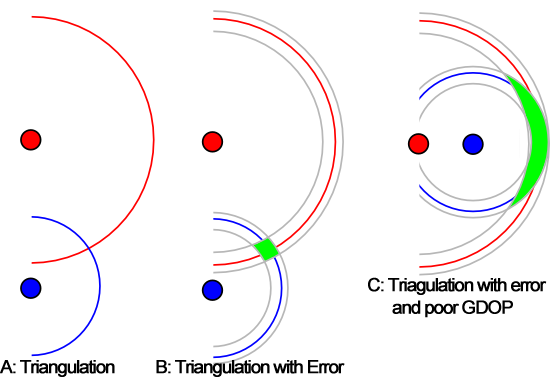
\includegraphics[width=.5\textwidth]{./pics_gps/dop.png}
  \end{center}
\vspace{-20pt}
  \caption{DOP en 2 dimensiones.}
\vspace{-50pt}
\label{fig:dop.png}
\end{wrapfigure}

El método que utiliza el GPS para determinar su ubicación consiste básicamente en:
\begin{enumerate}
\item Determinar la distancia $r_i$ a cada satélite $S_i$, cuya posición es $P_i$.
\item Repetir el paso anterior para cada satélite disponible.
\item Intersectar las ``cáscaras'' de las esferas de centros $P_i$ y radios $r_i$.
\end{enumerate}

Las ``cáscaras'' de las esferas no serán de ancho despreciable, ya que hay un cierta incertidumbre asociado a los datos. Esto implica que la intersección será un volumen, en lugar de un punto. La geometría de la distribución de los satélites determinará el tamaño de este volumen, y por lo tanto la incertidumbre en la determinación de la posición. En la figura \ref se muestra un ejemplo ilustrativo, en dos dimensiones.

El DOP es el cociente entre la exactitud de la ubicación y exactitud de la medida\cite{bib:sat-pos}:
\begin{equation*}
  \sigma = \sigma_o.DOP
\vspace{-10pt}
\end{equation*}
donde
\begin{itemize}
\item $\sigma$: Exactitud de la medida.
\item $\sigma_o$: Exactitud de la posición. 
\end{itemize}

 Básicamente, el DOP representa la sensibilidad de localización frente a errores en las medidas, o sea, cuanto te vas a perder si te llego una medida equivocada. Cuanto más bajo sea el DOP, mejor. En la tabla \ref{tab:dop} se muestra como interpretar valores típicos\cite{bib:sat-dop-values}.

\begin{table}[H]
\begin{center}
\begin{tabular}{|l|c||p{7cm}|}
\hline
\rowcolor[gray]{0.9}
1 & Ideal & Máxima exactitud posible.\\
\rowcolor[gray]{0.95}
1-2 & Excelente & La exactitud a este nivel se considera suficiente para casi cualquier aplicación.\\
\rowcolor[gray]{0.9}
2-5 & Bueno & Este nivel marca el mínimo apropiado para navegación. \\
\rowcolor[gray]{0.95}
5-10 & Moderado & Las medidas se pueden utilizar, pero es recomendado buscar un lugar con cielo más abierto. \\
\rowcolor[gray]{0.9}
10-20 & Regular & Solo se deben usar los datos para estimaciones de muy poca precisión. \\
\rowcolor[gray]{0.95}
$>$20 & Malo & A este nivel, las exactitud de las medidas puede tener un error de hasta 300m, deben descartarse. \\
\hline
\end{tabular}
\caption{Interpretación de los valores de DOP.}
\label{tab:dop}
\end{center}
\end{table}

El GPS envía información sobre:
\begin{itemize}
\item \textit{HDOP} - DOP horizontal:
  \begin{equation}
    \label{eq:hdop}
    HDOP = \sqrt{\sigma_{easting}^2+\sigma_{northing}^2}    
  \end{equation}
\item \textit{VDOP} - DOP vertical:
  \begin{equation}
    \label{eq:vdop}
    VDOP = \sqrt{\sigma_{altitud}^2}
  \end{equation}
\item \textit{PDOP} - DOP de la posición:
  \begin{equation}
    \label{eq:pdop}
    PDOP = \sqrt{\sigma_{easting}^2+\sigma_{northing}^2 + \sigma_{altitud}^2}
  \end{equation}
\end{itemize}

Esta información se puede utilizar en el algoritmo de control, para ponderar los datos provenientes del GPS.

\bibliographystyle{plain} 
\bibliography{biblio}
\end{document}
